\documentclass[conference]{IEEEtran}
\IEEEoverridecommandlockouts
% The preceding line is only needed to identify funding in the first footnote. If that is unneeded, please comment it out.
\usepackage{cite}
\usepackage{amsmath,amssymb,amsfonts}
\usepackage{algorithmic}
\usepackage{graphicx}
\usepackage{textcomp}
\usepackage{xcolor}
\def\BibTeX{{\rm B\kern-.05em{\sc i\kern-.025em b}\kern-.08em
    T\kern-.1667em\lower.7ex\hbox{E}\kern-.125emX}}

\setlength\arraycolsep{2pt}

\begin{document}

\title{State estimation and inertial measurement units\\
}

\author{\IEEEauthorblockN{1\textsuperscript{st} mzandtheraspberrypi}
\IEEEauthorblockA{\textit{Computer Science Department} \\
\textit{Some School of Engineering}\\
London, England}
}

\maketitle

\begin{abstract}
Inertial measurement units have a long history of being used for state estimation. Unfortunately, they accumulate error as they are used which can be mitigated by fusing another sensor's data, for instance with a Kalman filter. For the project, a dataset of IMU measurements including accelerometer, gyroscope, and magnetometer data was found and studied. A method to measure orientation without accumulation of errors over time was implemented. The princple assumption is that of no linear acceleration acting on the object except gravity though this strong assumption is somewhat mitigated by model design. Simulation of the method on the dataset was conducted. Finally, a novel compass was designed that uses a live sensor with the model to estimate orientation in 3d-space using an extended kalman filter.
\end{abstract}

\begin{IEEEkeywords}
state estimation, imu, compass
\end{IEEEkeywords}

\section{Literature Review}
\subsection{State Estimation and Inertial Measurement}
State estimation is a vital field of study for the control of dynamical systems. The inertial measurement unit, or IMU, is a sensor that has been widely used in state estimation.
Tazartes points out that an early example of a system using inertial measurement was the system used by the V2 rockets developed by Nazi Germany \cite{b1}. In the late 1940s and 50s, much research
was undergone and inertial navigation systems were used in fighter jets, before in 1968 the first inertial navigation system for commercial aircraft was certified \cite{b1}. Before the sensor was widely and cheaply available,
practitioners had to rely on other sensors. For example, in the problem of Satellite Rendezvous in 1960, Clohessy and Wiltshire suggested using a ground based radar system to track the initial satellite,
and a further infrared homing system to complete rendezvous \cite{b2}. H. Black in 1964 proposed a passive system using solar attitude detectors to determine the attitude of a satellite \cite{b3}.

One drawback to inertial measurement systems is their propensity to accumulate errors over time. If we have white noise in our x-axis linear acceleration estimate, we integrate to get to velocity and error grows quadratically. We integrate to get to position and error grows cubically. One study in 1973 found that 45 minute flights using a three-axis inertial measurement system accumulated errors of $\pm 2^{\circ}$ \cite{b4}. Over longer periods of time this error can accumulate even more significantly. In 1966, Friedlander proposed using the Kalman filter to fuse celestial sensors with inertial measurement, "significantly reducing the long term effects of inertial gyro and accelerometer errors" \cite{b5}.

Fast forward to today and Micro-Electro-Mechanical Systems (MEMS) IMUs are cheaper, more compact, and require less processing power than earlier IMUs, leading to widespread usage \cite{b6}. In robotics, we often see applications fusing IMU data with other sensors to solve for IMU drift error and synergize with other sensors. For example, in visual-inertial odometry (VIO) the state including pose and velocity of an agent is estimated using the input of camera and IMU which are both cheap sensors \cite{b7}. Landmarks from the camera can be used to estimate state and fused with estimates from the IMU (loosely-coupled) or IMU measurements can be used to predict location of features (tightly-coupled) often using the extended Kalman filter \cite{b7}. Another example is lidar inertial odometry, where IMU data is fused with Lidar data, de-skewing it, and features from the Lidar are used to estimate poses \cite{b8}. A commonality in VIO and lidar inertial odometry is that both approaches take advantage of the high update rate of the IMU and that measurements don't depend on the surrounding scene, fusing it with other sensors that may not have those characteristics but have other characteristics that mitigate IMU weak-points like tendency to accumulate drift \cite{b7} \cite{b8}.

\subsection{Summary}
As we have seen, IMUs are an important sensor in state estimation and in state estimation for legged robots. IMUs have some drawbacks in terms of drift, but this can be mitigated by fusing with other sensor data \cite{b5} \cite{b7} \cite{b12}.

\section{Project Overview}
This paper focuses on the use of inertial measurement units for orientation estimation. A model is developed to estimate x, y, and z rotation, and applied to a live sensor setup to demonstrate applications using an extended kalman filter.

\section{Problem Setup}

How do we take a nine degree of freedom inertial measurement unit, including an accelerometer, a gyroscope, and a magnetometer, and use this to get position, velocity, and orientation? Traditional methods of double integrating linear angular acceleration to get to orientation accumulate drift and error over time. We will use an approach similar to \cite{b19} and \cite{b21} that uses the gravity vector in tandem with the earth's magnetic field vector to obtain static state estimates of orientation. This avoid drift accumulation in the orientation estimate. We can also avoid errors by fusing the output of the gyroscope measurements and the orientation estimate from the digital compass to get a better estimate than if we were to rely on just one method. This helps us be a bit more resilient to the assumption of zero linear acceleration.

\section{Methods}

\subsection{Orientation}

We define our world coordinate system so that the x axis aligns with magnetic north, the y axis aligns with magnetic east, and the z-axis points down.  

We have outputs of $a_{acc}$ from the accelerometer measuring linear acceleration, $H_{mag}$ from the magnetometer measuring the Earth's magnetic field, and $\omega_{gyro}$ angular acceleration from the gyroscope. We will obtain orientation from the accelerometer's x and y data, in combination with the magnetometer data, assuming little to no angular or linear acceleration. We will also get an orientation estimate from the double integral of angular acceleration. We will fuse this all together in an extended Kalman filter to get better estimates than we could for just one of the methods as per Fig \ref{fig:ekf}.

\begin{figure}[h!]
  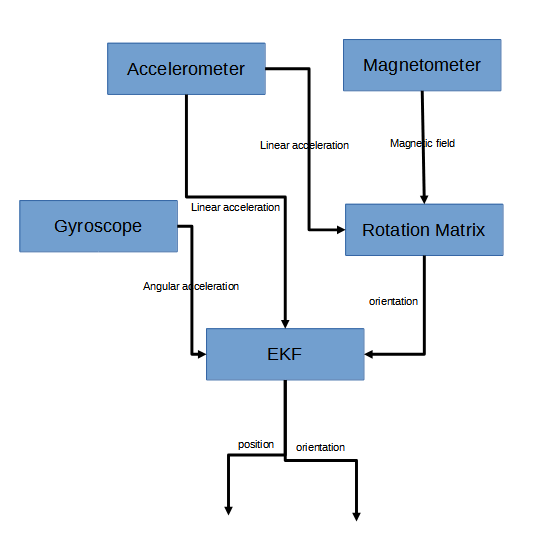
\includegraphics[width=\columnwidth]{fig_2_ekf.png}
  \caption{Sensors and EKF System}
  \label{fig:ekf}
\end{figure}


We use Euler angle formulations with y rotation, roll ($\phi$), x rotation, pitch ($\theta$), and z rotation, yaw ($\psi$), and for estimation of position and velocity we will use a similar method to \cite{b18} and \cite{b21}. We define gravity as per \eqref{eq:grav} where g represents the gravitational constant.


Similar to \cite{b19} gravity of the world frame relates to gravity in the body frame as per \eqref{eq:grav_body_to_world}, where $R_{w}^b$ denotes rotation matrix from world to the body frame. The rotation matrix from world to the body frame can be defined in \eqref{eq:rotation_world_body}, where c represents cos() and s represents sin(). This expresses a rotation of pitch, then roll, then yaw, or x, y, z, where the order matters.

\begin{align}
g_w =& \begin{bmatrix}0& 0& -g\end{bmatrix}^T \label{eq:grav}\\
g_w =& R_{b}^w g_b \label{eq:grav_body_to_world} \\
(R_{w}^b) =& \begin{bmatrix} c\theta c\psi& c\theta s\psi& -s\theta\\
					  s \phi s\theta c\psi - c \phi s\psi& s\phi s\theta s\psi + c\phi c\psi& s \phi c \theta\\
					 c \phi s \theta c \psi + s \phi s \psi& c \phi s \theta s\psi - s \phi c\psi& c \phi c \theta	\end{bmatrix}\label{eq:rotation_world_body}
\end{align} 

The accelerometer gives us gravitational accelerations in the robot body reference frame. We can relate the robot body gravitational acceleration to the world acceleration via \eqref{eq:gravity_world_to_body}, assuming the body is in a steady state with respect to acceleration.
\begin{align}
g_b =& R_w^b g_w, \text{where } R_w^b = (R_b^w)^T\\
g_b =& \begin{bmatrix} g_{bx}\\ g_{by}\\ g_{bz} \end{bmatrix} = R_{w}^b g_w = (-g) \begin{bmatrix} -sin \theta \\ sin \phi cos \theta \\ cos \phi cos \theta \end{bmatrix} \label{eq:gravity_world_to_body}
\end{align}

We can calculate $\phi$ and $\theta$ as per Fig \ref{fig:pitch}, with reference only to earth's gravitational vector avoiding accumulation and drift errors, but assuming litttle to no acceleration apart from gravity as per \cite{b19}.
\begin{align}
\phi =& arctan \left( \frac{g_{by}}{g_{bz}} \right)\\
\theta =& arctan \left( \frac{ - g_{bx}}{\sqrt{g_{by}^2 + g_{bz}^2}} \right )
\end{align}

\begin{figure}[h!]
  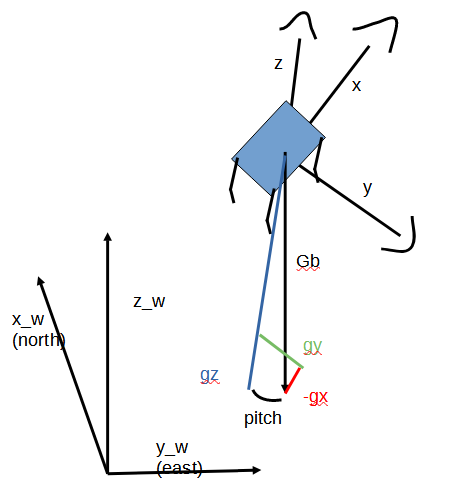
\includegraphics[width=\columnwidth]{fig_1_pitch.png}
  \caption{World Frame vs Robot Frame}
  \label{fig:pitch}
\end{figure}

With regards to yaw, we will use the three components of earth's magnetic field vector and transform the main plane of the magnetometer into the horizontal plane in the world frame using roll and pitch. Then we can calculate yaw, using \eqref{eq:yaw}, because after applying pitch and roll, yaw is all that is left.

\begin{align}
H^{hor} =& \begin{bmatrix} H_x^{hor}& H_y^{hor}& H_{z}^{hor}\end{bmatrix}^T = R(y, \theta) R(x, \phi) H^w \nonumber \\
R_w^b =& R(z, \psi) R(y, \theta) R(x, \phi)\\
\psi =& arctan(H_y^{hor} / H_x^{hor})\label{eq:yaw}
\end{align}

We've solved for the orientation without using integration and accumulating errors and drift. That said, this assumes zero or small rotation and translational acceleration so we isolate acceleration to just gravity.

\subsection{State Model and Dynamics}

Similar to \cite{b21} we define the state transition model for orientation by adding the change in angular rotation to the current orientation in \eqref{eq:state_transition_eq}. We can calculate angular rotation in the world frame with \eqref{eq:angular_rates_world_eq}.

\begin{align}
\begin{bmatrix} 
\theta_{t}^{w}\end{bmatrix} =& \begin{bmatrix} 
\theta_{t-1}^{w} + \delta t R_b^{\prime w}(\theta_{t-1}) \omega_{t-1}^b \end{bmatrix} \label{eq:state_transition_eq}\\
\begin{bmatrix} \omega_x^b\\ \omega_y^b\\ \omega_z^b \end{bmatrix} =& \begin{bmatrix} \omega_x^w\\ 0\\ 0\end{bmatrix} + R^T(x, \phi) \begin{bmatrix} 0\\ \omega_x^w\\ 0\end{bmatrix} \\
& + R^T(x, \phi) R^T(y, \theta) \begin{bmatrix} 0\\ 0\\ \omega_x^w \end{bmatrix} \\
\begin{bmatrix} \omega_x^w\\ \omega_y^w\\ \omega_z^w \end{bmatrix} =& R_b^{'w} (\theta) \omega^b\\
=& \begin{bmatrix} 1& sin\phi tan\theta& cos\phi tan\theta\\
			     0& cos \phi& -sin\phi\\
			    0& sin\phi / cos \theta& cos\phi/cos\theta \end{bmatrix} \begin{bmatrix} \omega_x^b\\ \omega_y^b\\ \omega_z^b \end{bmatrix}  \label{eq:angular_rates_world_eq}
\end{align}

State matrix only looking at the orientation. Hopefully more correct.


Substituting equation \ref{eq:angular_rates_world_eq} for the rotation from body to world, and doing the matrix multiplication with the angular velocities in body frame.
\begin{align}
\begin{bmatrix} 
\theta_{x_{t}}^{w}\\
\theta_{y_{t}}^{w}\\
\theta_{z_{t}}^{w}\end{bmatrix} =& \begin{bmatrix} 
\theta_{x_{t-1}}^{w} + \delta t (\omega_{x_{t-1}}^b + sin\phi tan \theta \omega_{y_{t-1}}^b + cos\phi tan\theta \omega_{z_{t-1}}^b) \\
\theta_{y_{t-1}}^{w} + \delta t (cos\phi \omega_{y_{t-1}}^b - sin\phi \omega_{z_{t-1}}^b) \\
\theta_{z_{t-1}}^{w} + \delta t (sin\phi  \omega_{y_{t-1}}^b / cos \theta + cos\phi \omega_{z_{t-1}}^b  / cos\theta) \end{bmatrix} \nonumber
\end{align}

This is non-linear, so we will take the jacobian, the derivative with respect to each element of the state matrix, and use an extended kalman filter. A will be 3x3, where ith row looks at the equation for ith element of state matrix, and each jth column is derivative of ith equation element with respect to jth element in state matrix.

\begin{align*}
\phi =  \theta_{x_{t}}^{w}, \theta =&  \theta_{y_{t}}^{w}, \psi =  \theta_{z_{t}}^{w}\\
A[0][0] =& \frac{\partial \theta_{x_{t}}^{w}}{\partial \theta_{x_{t}}^{w}}\\
A[0][0] =& 1 + \delta t cos\phi tan\theta \omega_{y_{t-1}}^b - \delta t sin\phi tan\theta  \omega_{z_{t-1}}^b \\
A[0][1] =& \frac{\partial \theta_{x_{t}}^{w}}{\partial \theta_{y_{t}}^{w}}\\
A[0][1] =& \delta t sin\phi (tan^2\theta + 1) \omega_{y_{t-1}}^b + \delta t cos\phi (tan^2\theta + 1)  \omega_{z_{t-1}}^b \\
A[0][2] =& \frac{\partial \theta_{x_{t}}^{w}}{\partial \theta_{z_{t}}^{w}}\\
A[0][2] =& 0 \\
A[1][0] =& \frac{\partial \theta_{y_{t}}^{w}}{\partial \theta_{x_{t}}^{w}}\\
A[1][0] =& \delta t (-sin\phi) \omega_{y_{t-1}}^b + \delta t (-cos\phi) \omega_{z_{t-1}}^b  \\
A[1][1] =& \frac{\partial \theta_{y_{t}}^{w}}{\partial \theta_{y_{t}}^{w}}\\
A[1][1] =& 1  \\
A[1][2] =& \frac{\partial \theta_{y_{t}}^{w}}{\partial \theta_{z_{t}}^{w}}\\
A[1][2] =& 0\\
A[2][0] =& \frac{\partial \theta_{z_{t}}^{w}}{\partial \theta_{x_{t}}^{w}}\\
A[2][0] =&  \delta t cos\phi \omega_{y_{t-1}}^b / cos \theta -  \delta t sin\phi \omega_{z_{t-1}}^b / cos\theta \\
A[2][1] =& \frac{\partial \theta_{z_{t}}^{w}}{\partial \theta_{y_{t}}^{w}}\\
A[2][1] =&  \delta t sin\phi \omega_{y_{t-1}}^b (\frac{1}{cos^2 \theta})(sin\theta)  + \delta t cos\phi \omega_{z_{t-1}}^b (\frac{1}{cos^2 \theta})(sin\theta) \\
A[2][2] =& \frac{\partial \theta_{z_{t}}^{w}}{\partial \theta_{z_{t}}^{w}}\\
A[2][2] =& 1 \\
\end{align*}


For the measurement model, let's assume static state. We could flesh this out further by making our acceleration measurement equal to linear, rotational, and gravity vector. But let's keep it simple for now. In the below, we model measurements of yaw from magnetometer calculation, and accelerometer observations.
\begin{align}
y_t(\theta) = \begin{bmatrix} \psi_m \\ a_x^b \\  a_y^b \\  a_z^b \end{bmatrix} =& \begin{bmatrix} \psi\\
															 -g (-sin \theta)\\
													              -g sin \phi cos \theta \\
													               -g cos \phi cos \theta \end{bmatrix} \nonumber
\end{align}

\begin{align*}
\theta_{x_{t}}=&\phi, \theta_{y_{t}}=\theta, \theta_{z_{t}}=\psi \\
C[0][0] = & 0 \\
C[0][1] = & 0 \\
C[0][0] =& 1\\
C[1][0] = & 0 \\
C[1][1] = & -g (cos\theta) \\
C[1][2] = & 0 \\
C[2][0] = & g cos\theta cos\phi \\
C[2][1] = & -g sin\phi(sin\theta)\\
C[2][2] = & 0\\
C[3][0] = & -g (sin\phi) cos\theta\\
C[3][1] = & -g cos\phi (sin\theta)\\
C[3][2] = & 0\\
\end{align*}

\section{Results}

The results showed that the model fits reasonably well to the ground truth given in the dataset \cite{b20}.  There is some jumping and some divergence where trig jumps are unaccounted for. There was some uncertainty regarding coordinate systems in the dataset, and hence this is corrected in the live model.  
\begin{figure}[h!]
  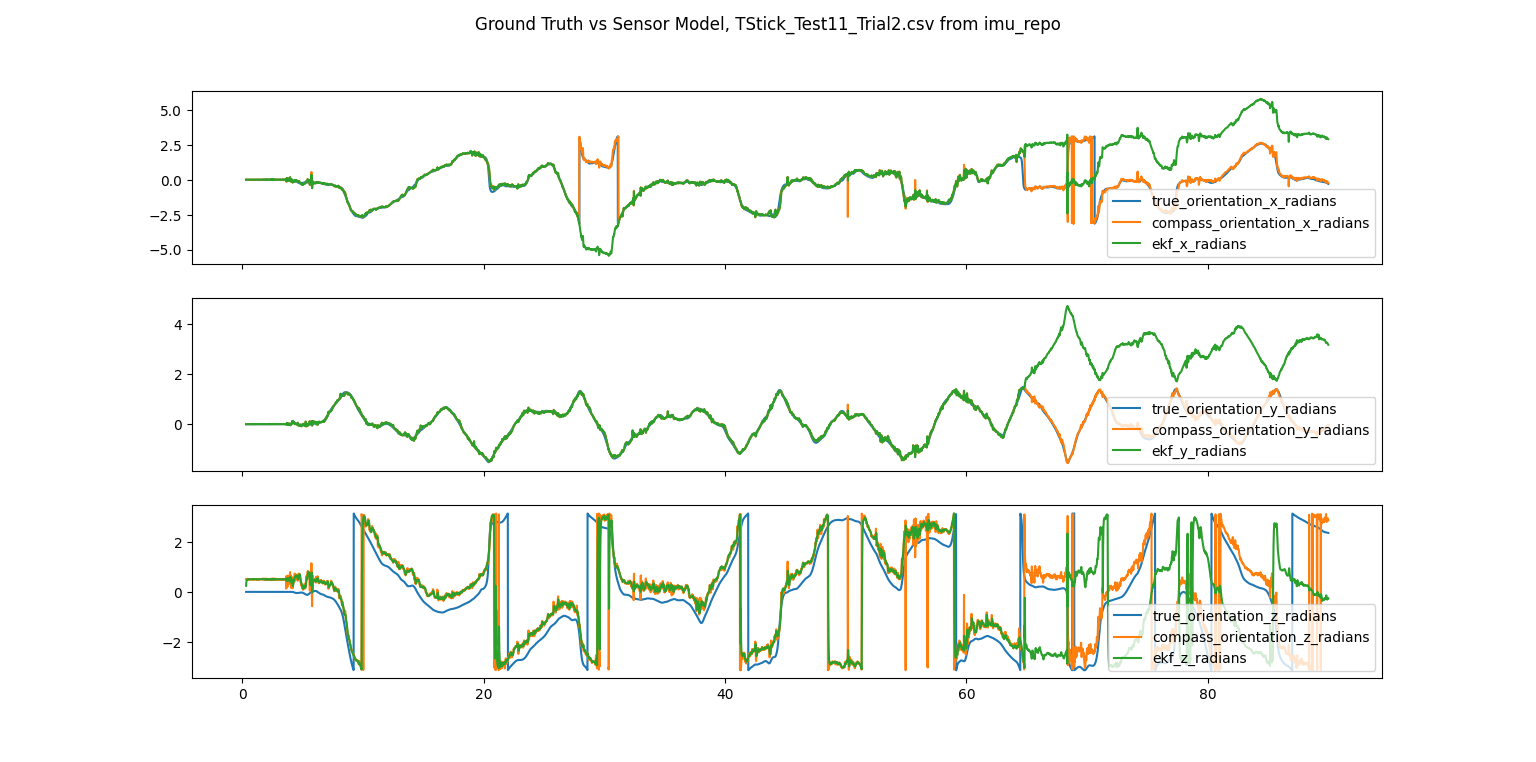
\includegraphics[width=\columnwidth]{estimate_vs_ground_truth.png}
  \caption{True Orientation vs Model Estimate}
  \label{fig:true_orientation_vs_estimate}
\end{figure}

\section{Live Model}

A digital compass was designed and this model was implemented on a raspberry pi 4 connected to a Bosch BNO055 sensor development board from Adafruit. The model works reasonably well. The screen shows the world coordinate frame and even as the sensor is rotated in 3-dimensions x aligns fairly well with magnetic north.  
\begin{figure}[h!]
  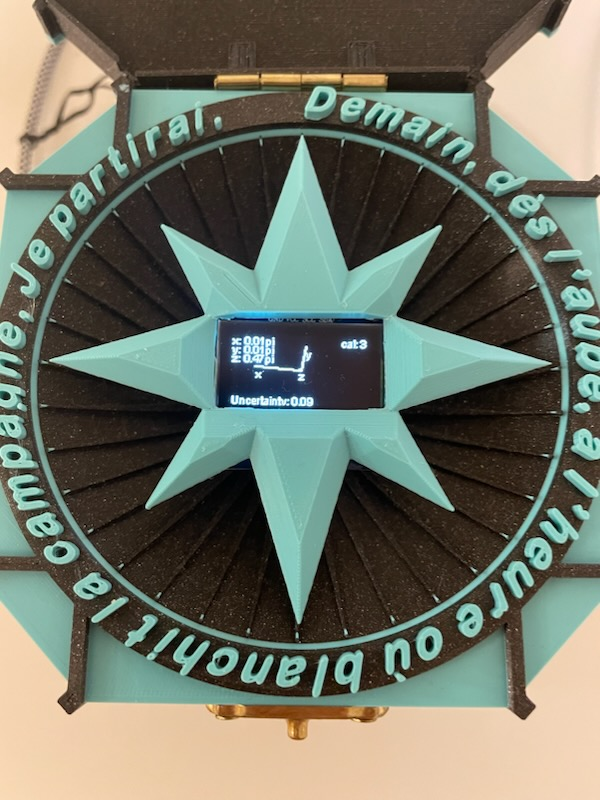
\includegraphics[width=\columnwidth]{IMG_20231012_140921.jpg}
  \caption{Digital Compass}
  \label{fig:compass_picture}
\end{figure}

\subsection{Lessons Learned and Next Steps}

The authors learned some valuable lessons from this project. Namely, well defining coordinate systems of the model and the sensor as well as unit conventions are vital when deploying on live sensors.

In terms of next steps, this model could be extended to estimate position, velocity, and acceleration. More work could also be done on calibration and on quantifying performance.


\begin{thebibliography}{00}
\bibitem{b1} D. Tazartes, (2014). ``An historical perspective on inertial navigation systems,`` 1-5. 10.1109/ISISS.2014.6782505. 
\bibitem{b2} W.H. Clohessy, R.S. WILTSHIRE, ``Terminal guidance system for satellite rendezvous,`` J.Aerosp. Sci. 27 (9) (1960) 653–658, http://dx.doi.org/10.2514/8.8704.
\bibitem{b3} H.D. Black, ``A passive system for determining the attitude of a satellite,`` AIAA Journal 1964 2:7, 1350-1351
\bibitem{b4} Wolf, Thomas D., and Robert C. McCracken. ``Ground and flight experience with a strapdown inertial measuring unit and a general purpose airborne digital computer,`` No. H-735. 1973.
\bibitem{b5} Friedlander, Alan L. ``Analysis of an optimal celestial-inertial navigation concept for low-thrust interplanetary vehicles,`` No. NASA-CR-457. 1966.
\bibitem{b6} Ahmad, Norhafizan, Ghazilla, Raja Ariffin Raja, and Khairi, Nazirah M. ``Reviews on various inertial measurement unit (IMU) sensor applications,`` International Journal of Signal Processing Systems 1.2 (2013): 256-262.
\bibitem{b7} Scaramuzza, Davide, and Zichao Zhang. ``Visual-inertial odometry of aerial robots,`` arXiv preprint arXiv:1906.03289 (2019).
\bibitem{b8} H. Ye, Y. Chen and M. Liu, ``Tightly Coupled 3D Lidar Inertial Odometry and Mapping,`` 2019 International Conference on Robotics and Automation (ICRA), Montreal, QC, Canada, 2019, pp. 3144-3150, doi: 10.1109/ICRA.2019.8793511.
\bibitem{b9} Priyaranjan Biswal, Prases K. Mohanty, ``Development of quadruped walking robots: A review,`` Ain Shams Engineering Journal, Volume 12, Issue 2, 2021
\bibitem{b10} Raibert, Marc, et al. ``Bigdog, the rough-terrain quadruped robot.`` IFAC Proceedings Volumes 41.2 (2008): 10822-10825.
\bibitem{b11} Hutter, Marco, et al. ``Anymal-a highly mobile and dynamic quadrupedal robot.`` 2016 IEEE/RSJ international conference on intelligent robots and systems (IROS). IEEE, 2016.
\bibitem{b12} Bloesch, Michael, et al. ``State estimation for legged robots-consistent fusion of leg kinematics and IMU.`` Robotics 17 (2013): 17-24.
\bibitem{b13} Fink, Geoff, and Claudio Semini. ``Proprioceptive sensor fusion for quadruped robot state estimation.`` 2020 IEEE/RSJ International Conference on Intelligent Robots and Systems (IROS). IEEE, 2020.
\bibitem{b14} Buchanan, Russell, et al. ``Learning inertial odometry for dynamic legged robot state estimation.`` Conference on Robot Learning. PMLR, 2022.
\bibitem{b15} Wisth, David, Marco Camurri, and Maurice Fallon. ``Robust legged robot state estimation using factor graph optimization.`` IEEE Robotics and Automation Letters 4.4 (2019): 4507-4514.
\bibitem{b16} G. Fink and C. Semini, ``Proprioceptive Sensor Dataset for Quadruped Robots,`` IEEE Dataport, 2019, DOI:10.21227/4vxz-xw05
\bibitem{b17} G. Fink and C. Semini, (2019), ``Propioceptive Sensor Dataset for Quadrupeds,`` at the workshop on Visual-Inertial Navigation: Challenges and Applications in the IEEE/RSJ Internation Conference on Intelligent Robots and Systems (IROS), Macau, China, Nov. 2019, pp. 1–5
\bibitem{b18} Alatise, Mary B., and Gerhard P. Hancke. ``Pose estimation of a mobile robot based on fusion of IMU data and vision data using an extended Kalman filter`` Sensors 17.10 (2017): 2164.
\bibitem{b19} Zhao, He, and Zheyao Wang. ``Motion measurement using inertial sensors, ultrasonic sensors, and magnetometers with extended kalman filter for data fusion.`` IEEE Sensors Journal 12.5 (2011): 943-953.
\bibitem{b20} Szczesna, Agnieszka and Skurowski, Przemysław and Pruszowski, Przemyslaw and Peszor, Damian and Paszkuta, Marcin and Wojciechowski, Konrad. (2016). Reference Data Set for Accuracy Evaluation of Orientation Estimation Algorithms for Inertial Motion Capture Systems.
\bibitem{b21} Saito, A., Kizawa, S., Kobayashi, Y. et al. Pose estimation by extended Kalman filter using noise covariance matrices based on sensor output. Robomech J 7, 36 (2020). https://doi.org/10.1186/s40648-020-00185-y
\end{thebibliography}


\end{document}
